\chapter{Fazit}

\section{Beispiel für floats}

Zum Thema Platzierung von floats, sehen Sie sich bitte diese Seite an:\\
\url{https://tex.stackexchange.com/questions/39017}\\
\ \\
Hier erhalten beide floats die Platzierungsanweisung p und werden erwartungsgemäß beide auf eine gemeinsame Seite verschoben.

\Blindtext

% Ein Bild als figure:
% * es taucht im Bilderverzeichnis auf.
% * Sie können eine Bildunterschrift / caption vergeben.
% * Ein Kurztitel ist möglich.
% Sie können Präferenzen vergeben, wo das Bild angezeigt werden soll.
% Die Reihenfolge hat kein Gewicht, aber das Fehlen einer Option:
% h = here
% t = top of page
% b = bottom of page
% p = page for images
% H = (wenn float geladen ist) Anzeige hier erzwingen
\begin{figure}[p]
\centering
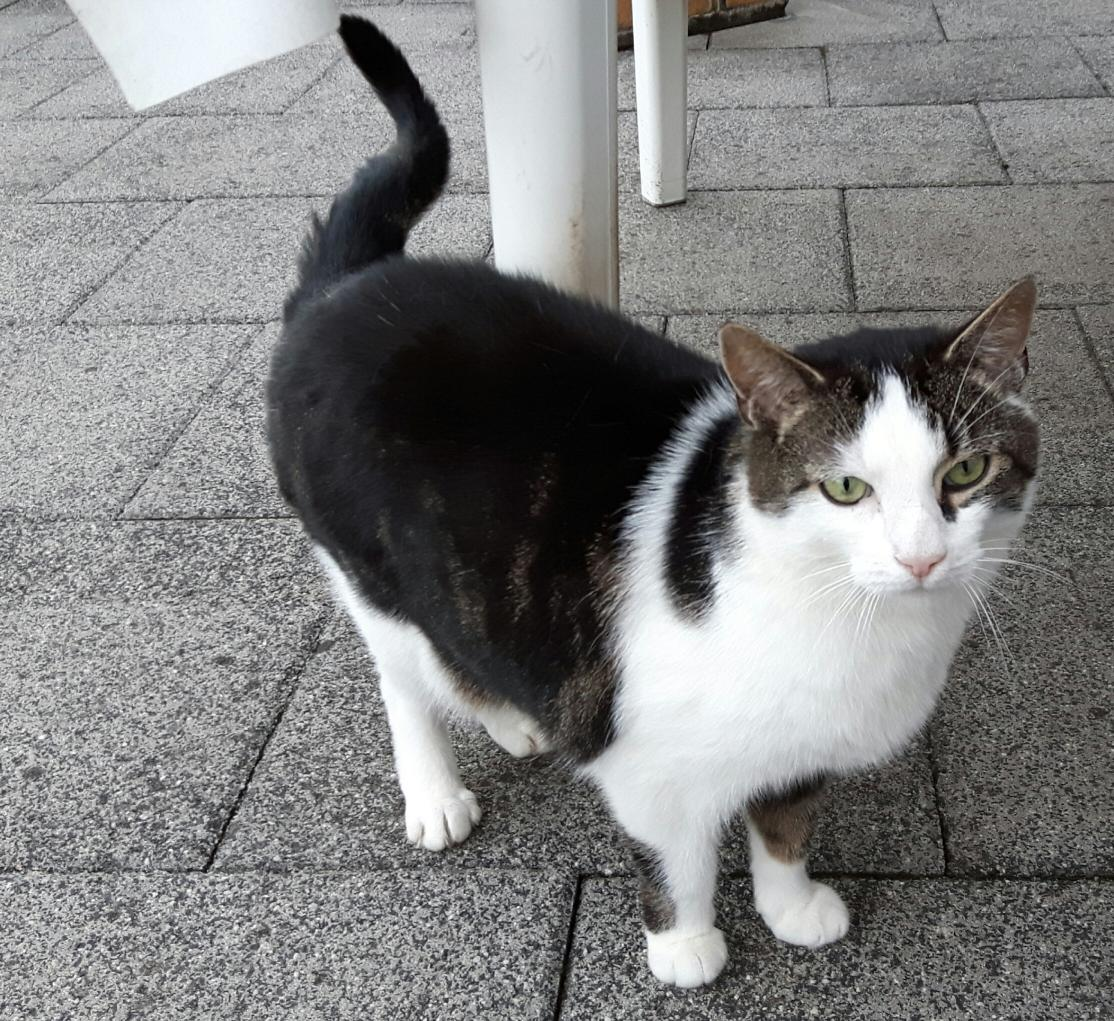
\includegraphics[scale=0.5]{img/Dala}
\label{figDala}
\caption[Kurztitel Katze]{Das ist die Katze Dala im Jahr 2018.}
\end{figure}

\Blindtext

\begin{figure}[p]
\centering
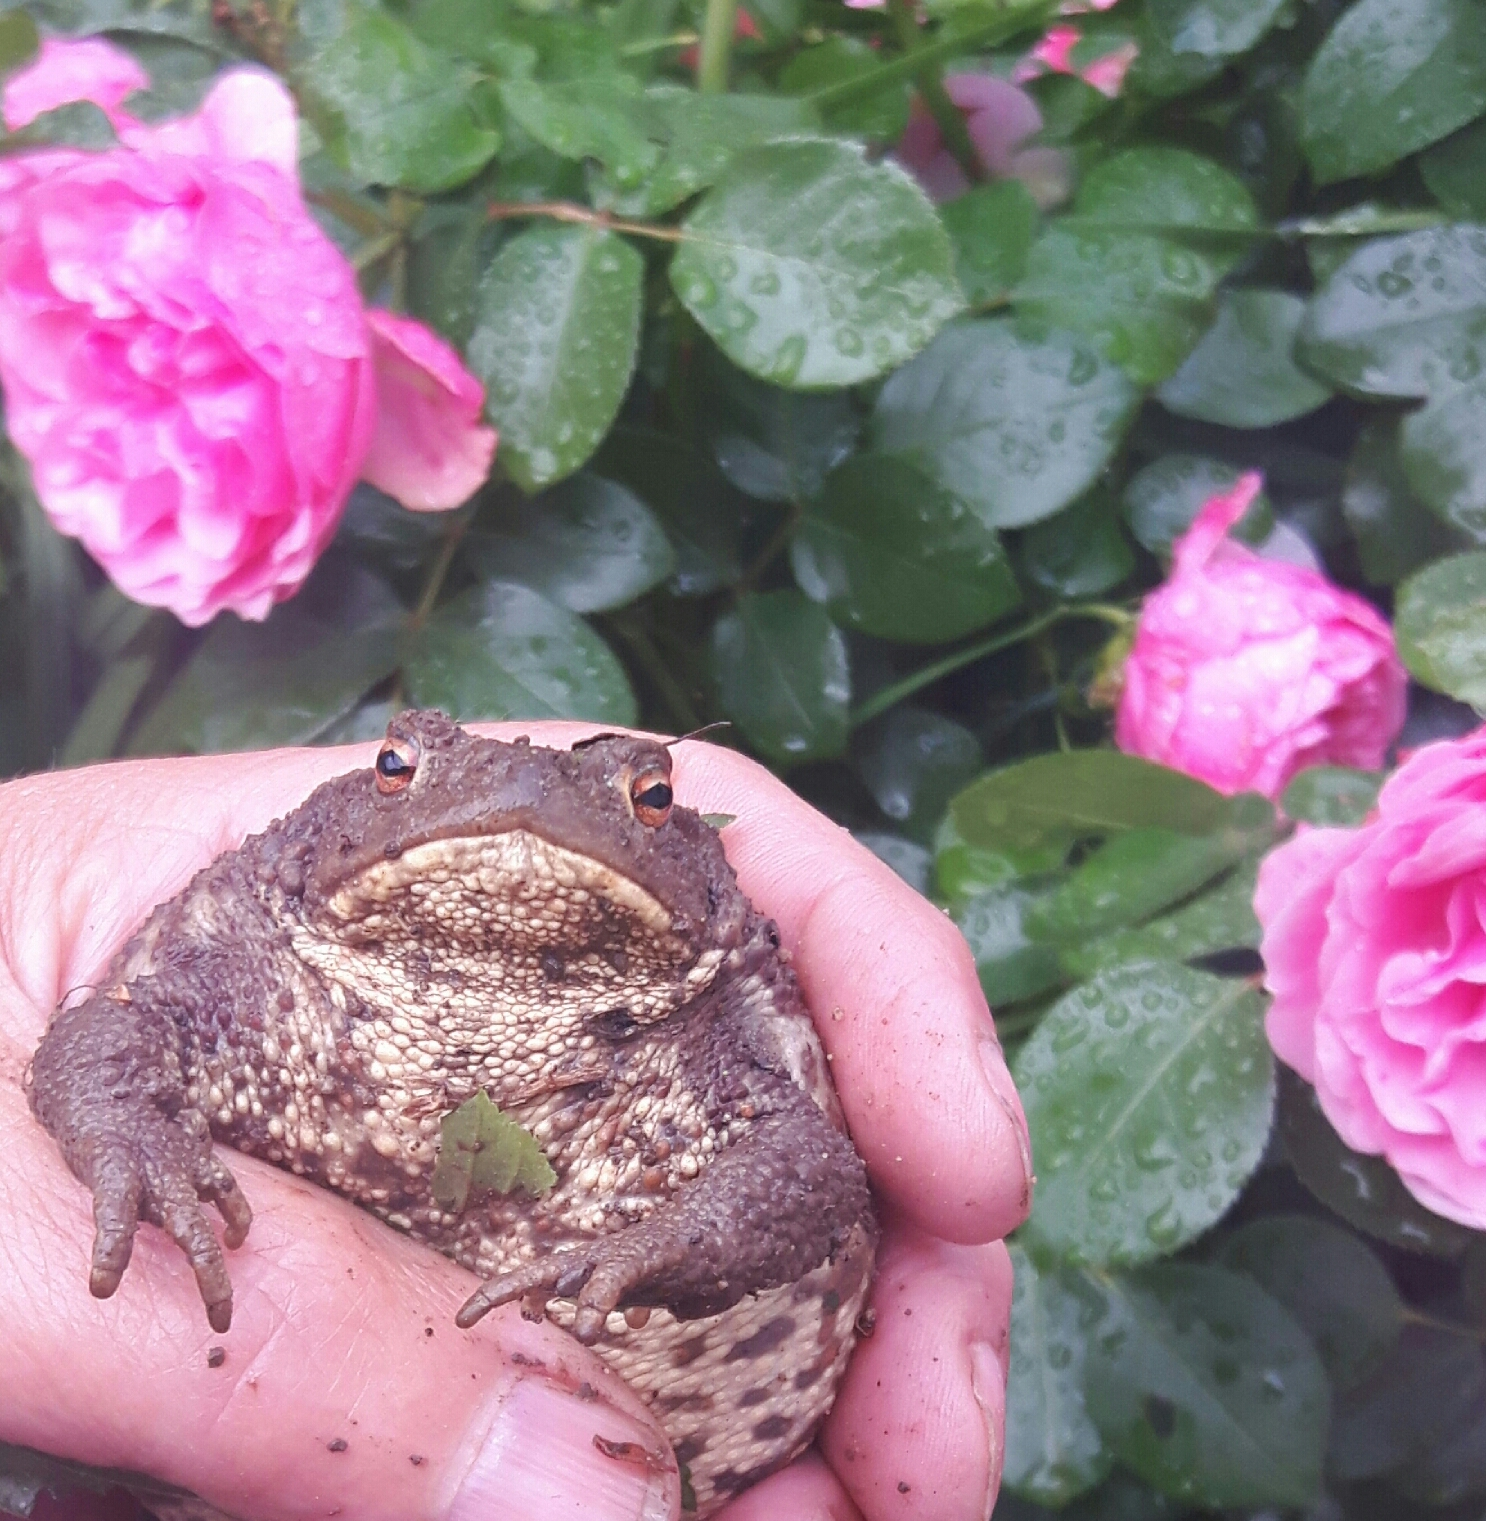
\includegraphics[width=0.4\textwidth]{img/toad}
\label{kroete}
\caption[Kurztitel Kröte]{Kröte, die sich in meinen Garten verirrt hat und zum nächsten Teich gebracht wurde.}
\end{figure}

\Blindtext




\section{Aufzählungen}

Aufzählungen sind eigene Umgebungen und lassen sich schachteln:

\begin{itemize}
\item abc
\item def  \begin{enumerate}
\item eins
\item zwei
\end{enumerate}
\end{itemize}






\url{http://www.uni-koeln.de}

